\documentclass{beamer}

\setbeamercovered{transparent}

\usepackage{pxfonts}
\usepackage{listings}
\title{Chapter 2: Number Systems and Codes
}
\subtitle{Lesson 2.3: Codes}
\author{Computer Fundamentals}
\institute{Second Edition}
 %\institute{\inst{1}Texas A\&M University \and \inst{2}Other University}
\date{\small{}}

% color
\definecolor{maroon}{RGB}{80,0,0} % A&M's primary color
\definecolor{332C2C}{RGB}{51,44,44} % A&M's primary support color, dark gray
\definecolor{5F574F}{RGB}{95,87,79} % A&M's secondary colors, light gray
\usecolortheme[named=maroon]{structure}
\setbeamercolor{frametitle}{fg=maroon,bg=white}
\setbeamercolor{primary}{fg=white,bg=maroon}
\setbeamercolor{secondary}{fg=white,bg=5F574F}

% headline
\setbeamertemplate{headline}{
\hbox{%
    \begin{beamercolorbox}[wd=0.5\paperwidth,ht=2.25ex,dp=1ex,left]{primary}
        \hspace*{2ex}\insertsectionhead % Section Title in Left
    \end{beamercolorbox}%
    \begin{beamercolorbox}[wd=0.5\paperwidth,ht=2.25ex,dp=1ex,left]{secondary}
        \hspace*{2ex}\insertsubsectionhead % Subsection Title in Right
    \end{beamercolorbox}}
\vskip0pt }

% footline
\setbeamertemplate{footline}{
\hbox{%
    \begin{beamercolorbox}[wd=.49\paperwidth,ht=2.25ex,dp=1ex,left]{primary}
        \hspace*{2ex}{Lesson 1.1: Introduction to Computers} % Something in Left
    \end{beamercolorbox}%
    \begin{beamercolorbox}[wd=.02\paperwidth,ht=2.25ex,dp=1ex,center]{primary}
        %\includegraphics[height=2.25ex,dp=2.25ex]{aTm08-box} % aTm Logo in the Middle
    \end{beamercolorbox}%
    \begin{beamercolorbox}[wd=.49\paperwidth,ht=2.25ex,dp=1ex,right]{primary}
        \insertframenumber{} / \inserttotalframenumber \hspace*{3ex} % Page numbers in Right
    \end{beamercolorbox}}
\vskip0pt }

\let\Tiny=\tiny



\begin{document}
\frame{\titlepage}

\section{Objectives}
\frame{\pause
On completion of this lesson you will know:\pause
\begin{itemize}
  \item Basic concepts of data information and codes\pause
\item	Representation of numeric data using binary numbers,\pause
\item	About BCD, EBCDIC, ASCII Codes\pause
\item About Unicode

\end{itemize}
}
\section{Data, Information and Codes}
\frame
{\pause
\begin{itemize}
\item Data are the names given to basic facts such as names and numbers. Unit-price is an examples of data.\pause
\item Information is processed data, that is, information is data which have been converted to a more useful form. For example total price = unit price � quantity sold. Here total price is information and unit price and quantity sold are data.\pause
\item Codes are used to reduce the volume of data. By coding, recording of data can be made sunoke laborious, less prone to error and the data become more manageable and easier to manipulate.
\end{itemize}
}

\section{Numeric Data Representation}
\frame
{\pause
\begin{itemize}

   \item Numeric data are represented in the computer using binary numbers. So anything which has to be stored in the memory must be converted into a binary form and then the bits can be used.\pause
   \item To store any positive integers the location is being filled with bits from right to left. The extra bits are filled up with 0s. To store $423_{10}$ in a memory location of word length of 16 bits, first convert $423_{10}$ into $110100111_2$ and fill the extra bits with 0s. \pause \centering {
        \begin{tabular}{|c|c|c|c|c|c|c|c|c|c|c|c|c|c|c|c|}
         \hline
         % after \\: \hline or \cline{col1-col2} \cline{col3-col4} ...
         0 & 0 & 0& 0& 0& 0& 0& 1& 1& 0& 1& 0& 0& 1& 1& 1\\
         \hline
         \end{tabular}
         }
 \end{itemize}

}

\section{Numeric Data Representation}
\subsection{Sign Magniture Representation}
\frame
{\pause \begin{itemize}
   \item The left most bit in the word represents the sign bit. If the left most bit is 0, the number stored in the word will be treated as a positive integer. On other hand if the left most bit is 1, then the number in the word will be treated as a negative integer. That bit is called the sign bit.\pause
   \item For example, storing +50 in a 16-bit word is as follows \pause \begin{tabular}{|c|c|c|c|c|c|c|c|c|c|c|c|c|c|c|c|}
        \hline
        % after \\: \hline or \cline{col1-col2} \cline{col3-col4} ...
        0 & 0 & 0& 0& 0& 0& 0& 0& 0& 0& 1& 1& 0& 0& 1& 0\\
        \hline
        \end{tabular}
\item For example, storing -50 in a 16-bit word is as follows
        \begin{tabular}{|c|c|c|c|c|c|c|c|c|c|c|c|c|c|c|c|}
        \hline
        % after \\: \hline or \cline{col1-col2} \cline{col3-col4} ...
        1 & 0 & 0& 0& 0& 0& 0& 0& 0& 0& 1& 1& 0& 0& 1& 0\\
        \hline
        \end{tabular}
        \item In the sign magnitue representation, the largest (i.e., positive) integer that can be stored in a 16-bit memory location is  $2^{15}-1$. Similarly the smallest (i.e., negative) integer that can be stored in a  16-bit memory location is  $-2^{15}$.
 \end{itemize}
}

\subsection{1's Complement Representation}
\frame
{\pause
\begin{itemize}
   \item Positive number is identical to that used in the sign magnitude system.\pause
   \item It consists of a left most sign bit in the leftmost position, followed by the magnitude bits.
   \item For a positive number, two representations are identical.\pause
   \item In case of negative numbers, the magnitude bits are represented by their 1's complement which is obtained by inverting each bit including the sign bit.\pause
   \item For example, the 1's complement of $25_{10}=11001_2$ is $00110_2$. And the 1's complement of $-5_{10}$ is $1010_2$.
  \end{itemize}
}
\subsection{2's Complement Representation}
\frame
{\pause
\begin{itemize}
   \item 2's complement representation of a - ve number is obtained by adding a 1 to the 1's complement of that number.

       Thus the 2's complement of $-50$ is
       \begin{tabular}{|c|c|c|c|c|c|c|c|c|c|c|c|c|c|c|c|}
        \hline
        % after \\: \hline or \cline{col1-col2} \cline{col3-col4} ...
        1 & 1 & 1& 1& 1& 1& 1& 1& 1& 1& 0& 0& 1& 1& 1& 0\\
        \hline
        \end{tabular}

  \end{itemize}
}

\subsection{Representation of Real Number}
\frame
{\frametitle{Fixed point representation}\pause

There are two most commonly used representations:
\begin{itemize}
   \item The position of decimal point is fixed which is assumed to be after the first 8 bits in this representation.\pause
       \item The first 8 bits store the integer portion of the number and the last 8 bits store the fractional part.\pause
       \item The bits in the integer part are filled from right to left and the remaining bits are padded with 0's.  The left most bit is reserved for the sign bit.\pause
       The representation of $-101001011.001001_2$ in the 16 bit word is as follows :
\begin{tabular}{|c|c|c|c|c|c|c|c|c|c|c|c|c|c|c|c|}
        \hline
        % after \\: \hline or \cline{col1-col2} \cline{col3-col4} ...
        1 & 1 & 0& 1& 0& 0& 1& 0& 1& 1& 0& 0& 1& 0& 0& 1\\
        \hline
        \end{tabular}
  \end{itemize}
}


\subsection{Representation of Real Number}
\frame
{\frametitle{Floating point representation}
\pause
There are two most commonly used representations:
\begin{itemize}
   \item It can be used to represent numbers in any positional number system.\pause
   \item It is written in the format $mb^e$, where $m$ is the mantissa, which is a signed fixed point number,  $e$ is the exponent, which is a signed integer and determines the actual position of the decimal point, $b$ is the base of the number.\pause

  \end{itemize}
\begin{figure}[ht!]
\centering
  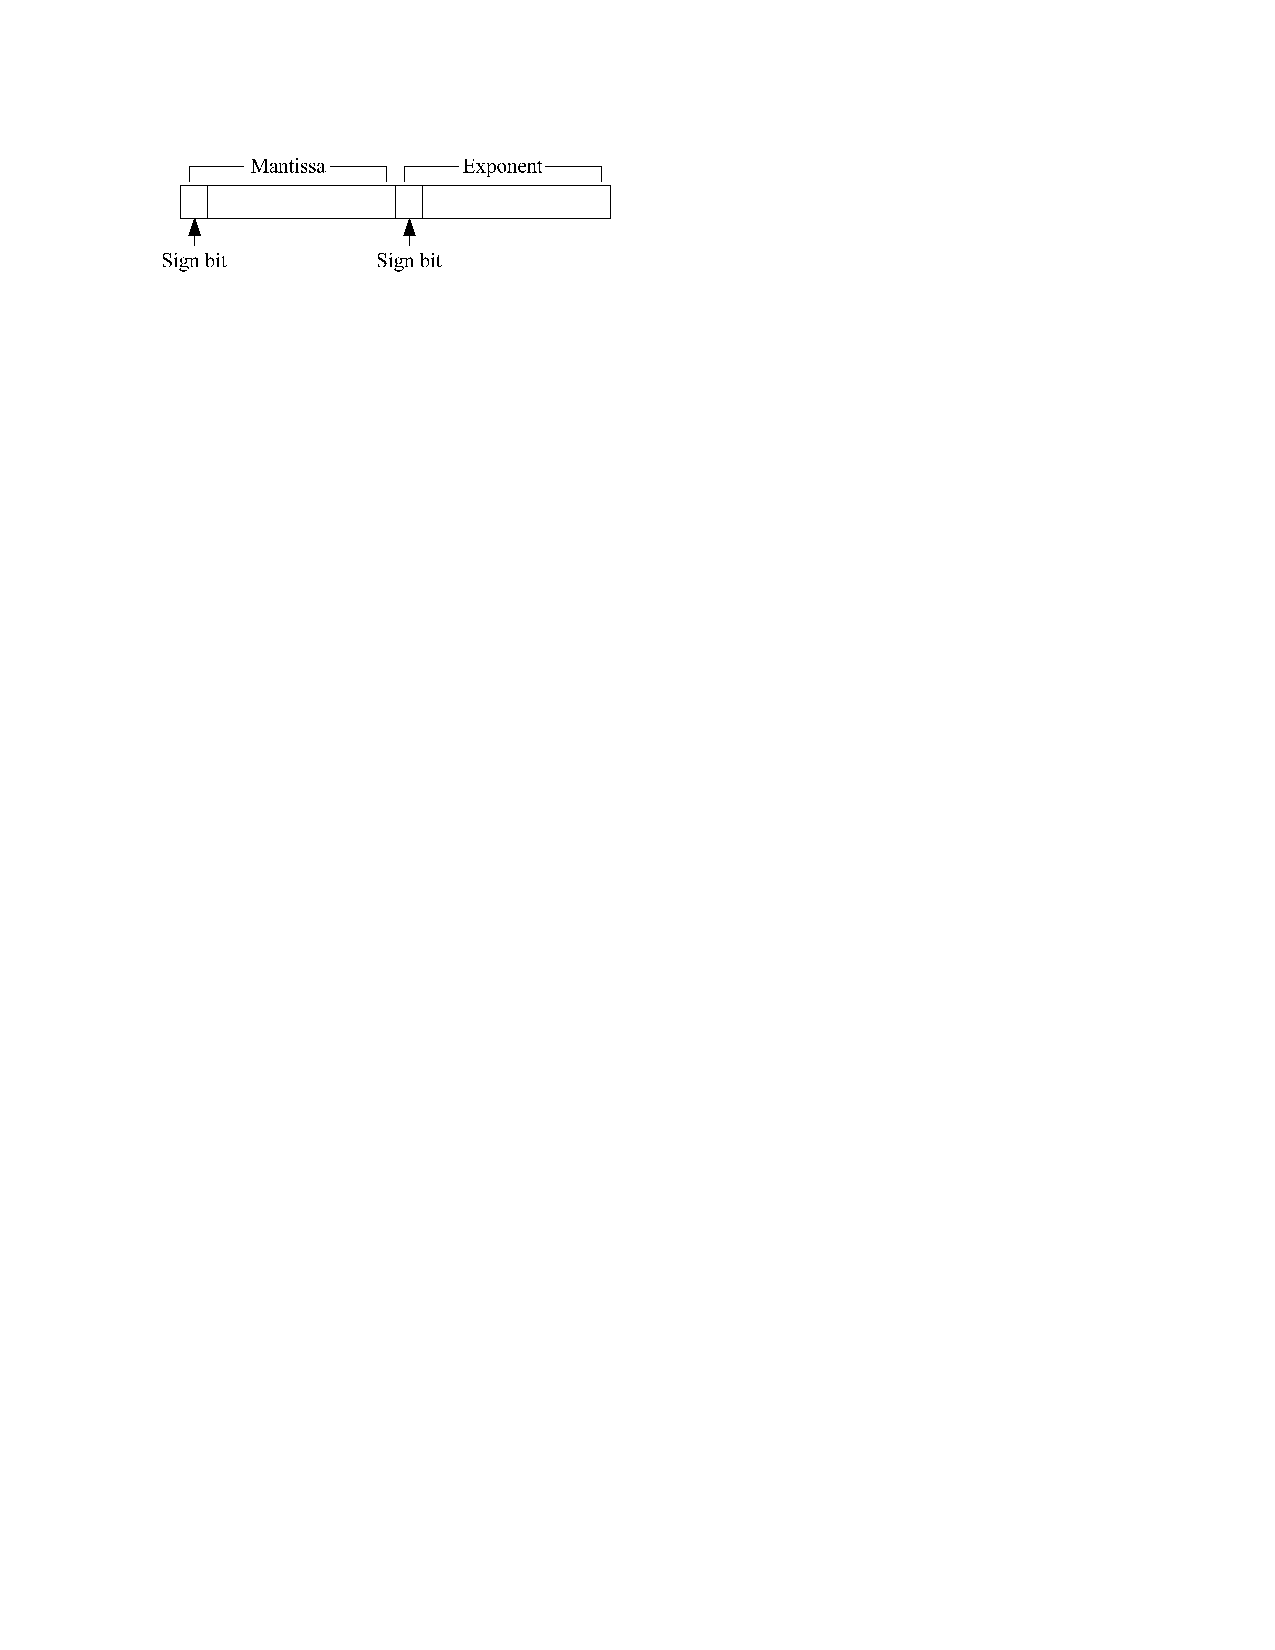
\includegraphics[width=8cm]{311}\\
\caption{2.3.2: Floating point representation}
\end{figure}
}

\section{BCD Code}

\frame
{\pause
\begin{itemize}
\item In the binary coded decimal (BCD) each decimal digit is represented by 4 bits. When only 4 bits are used a total of 16 configurations are possible.\pause
\item The 6 bits are used to represent each character (the four BCD numeric positions and two additional zone positions).\pause
\item When only 6 bits are used a total of 64 configurations are possible which means 64 different characters can be represented.\pause
\item For example,\pause
          \begin{tabular}{|c|c|c|c|}
        \hline
        % after \\: \hline or \cline{col1-col2} \cline{col3-col4} ...
        Character & Zone  & Digit & Octal \\ \hline
        A & 11&0001&61\\
        \hline
        \end{tabular}
\end{itemize}

}

\section{EBCDIC}

\frame
{\pause
\begin{itemize}
\item EBCDIC stands for extended binary coded decimal interchange code. \pause
\item In EBCDIC format, 8 bits are used to represent each character. \pause
\item In this code, it is possible to represent $256 (=2^8)$ different characters. It can be easily divided into two 4 bit groups. \pause
\item Each of these 4 bit groups can be represented by 1 hexadecimal digit.\pause
\item For example \pause
\begin{tabular}{|c|c|c|c|}
        \hline
        % after \\: \hline or \cline{col1-col2} \cline{col3-col4} ...
        Character & Zone  & Digit & Hexadecimal \\ \hline
        A & 1100&0001&C1\\
        \hline
        \end{tabular}
\end{itemize}
}


\section{ASCII}

\frame
{\pause
\begin{itemize}
\item American Standard Code for Information Interchange (ASCII) is a very widely used computer code. There are of two types: ASCII-7 and ASCII-8.\pause
\item ASCII-7 is a 7 bit code that allows $128(=2^7)$ different characters. The first 3-bits are used as zone bits and the last 4-bits indicate the digit. \pause
\item Microcomputers using 8-bits byte use the 7-bits ASCII by leaving the leftmost bit of each byte as a zero.  ASCII-8 is 8-bits code that allows $256 (=2^8)$ different characters.\pause
\item For example\pause
\begin{tabular}{|c|c|c|c|}
        \hline
        % after \\: \hline or \cline{col1-col2} \cline{col3-col4} ...
        Character & Zone  & Digit & Hexadecimal \\ \hline
        A & 100&0001&41\\
        \hline
        \end{tabular}
\end{itemize}
}






\section{Unicode}

\frame
{\pause
\begin{itemize}
  \item Unicode is a computing industry standard for the consistent encoding, representation and handling of text expressed in most of the world's writing systems.\pause
  \item It provides a unique number for every character as shown in Figure 2.3.3, no matter what the platform, no matter what the program, no matter what the language.\pause
\end{itemize}
     \begin{figure}[ht!]
\centering
  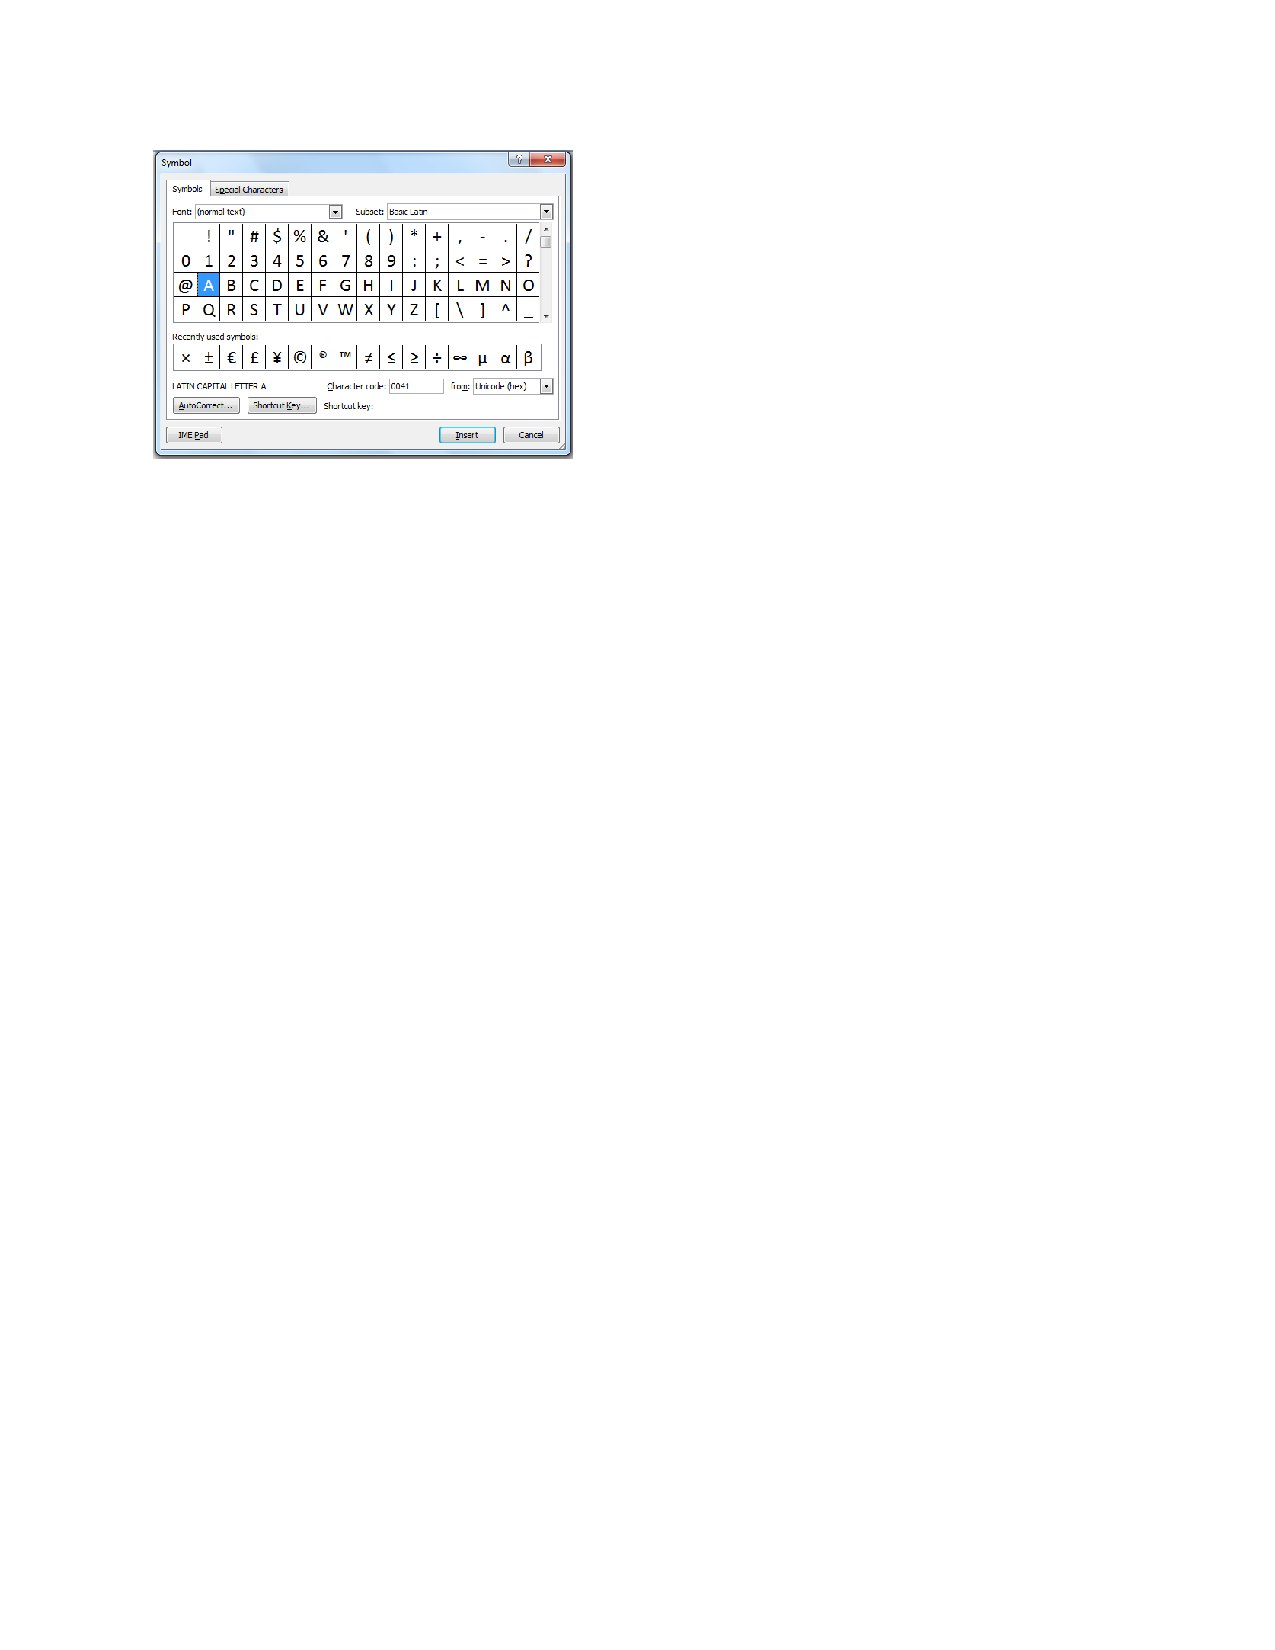
\includegraphics[width=6cm]{312}\\
\caption{2.3.3: Unicode}
\end{figure}

      }
\frame
{\pause
\begin{itemize}
  \item The Unicode Standard has been adopted by such industry leaders as Apple, HP, IBM, JustSystems, Microsoft, Oracle, SAP, Sun, Sybase, Unisys and many others.\pause
\item Unlike ASCII, which uses 7 bits for each character, Unicode uses 16 bits, which means that it can represent more than 65,000 unique characters. This is a bit of overkill for English and Western-European languages, but it is necessary for some other languages, such as Greek, Chinese and Japanese.\pause
\item Many analysts believe that as the software industry becomes increasingly global, Unicode will eventually supplant ASCII as the standard character coding format.\pause
\item The most recent Unicode version as of 2012 is Unicode 6.1.
\end{itemize}
}

\frame
{
\begin{itemize}

\pause
\item The different encodings implement Unicode.\pause
\item The most commonly used encodings are UTF-8 (or UCS Transformation Format-8), UTF-16 and UCS-2. UCS-2 uses a 16-bit code unit (two bytes) for each character but cannot encode every character in the current Unicode standard and it is now obsolete.\pause
\item UTF-8 uses one byte for any ASCII characters, and up to four bytes for other characters. UTF-16 extends UCS-2, using two 16-bit units to handle each of the additional characters.


\end{itemize}
}
\end{document}
